% !TeX root = main.tex
% --- PRÄAMBEL ---
% Satzspiegel, Schrift und Zeilenabstand entsprechen typischen Hochschulvorgaben
% (10–12 pt, 1,2- bis 1,4-facher Zeilenabstand). Mit den Vorgaben des eigenen
% Prüfers abgleichen: .claude/instructions/vorgaben.md
\documentclass[10pt, a4paper, parskip=half, ngerman, headings=small]{scrreprt}
% 10 pt, A4, Absätze mit halbem Zeilenabstand statt Einzug, kleinere Überschriften (KOMA-Script)

% --- SPRACHE & SCHRIFT ---
\usepackage[T1]{fontenc}               % Umlaute als eigene Glyphen: korrekte Silbentrennung, PDF-Suche und Kopieren
\usepackage[ngerman]{babel}            % deutsche Trennmuster, Datumsformat, Bezeichnungen ("Abbildung", "Inhaltsverzeichnis")
\usepackage{mathptmx}                  % Schrift Times
\usepackage{microtype}                 % Randausgleich und feine Zeichenabstände: weniger Überläufe über den rechten Rand
\setlength{\emergencystretch}{3em}     % letzte Reserve: schwierige Zeilen etwas dehnen statt überlaufen lassen
\usepackage{setspace}                  % Zeilenabstand einstellbar
\setstretch{1.3}                       % 1,3-facher Zeilenabstand (Vorgabe: 1,2 bis 1,4)
\setkomafont{disposition}{\normalcolor\bfseries} % Überschriften in Times statt KOMA-Standard (serifenlos)

% --- ABBILDUNGEN & LISTEN ---
\usepackage{graphicx}                  % \includegraphics für PNG- und PDF-Abbildungen
\usepackage{float}                     % Platzierung [H]: Abbildung exakt an der Stelle im Quelltext
\usepackage{enumitem}                  % Listenabstände je Liste einstellbar (sonst greift parskip=half zwischen \item)
\usepackage{xcolor}                    % Farben, hier für den grauen Rahmen in \screenshot

% Screenshot mit dezentem grauem Rahmen; optionales Argument = Gesamtbreite.
% Diagramme (assets/diagrams/*.png) ohne Rahmen mit \includegraphics einbinden.
\newcommand{\screenshot}[2][\textwidth]{%
    \setlength{\fboxsep}{4pt}%
    \setlength{\fboxrule}{0.4pt}%
    \fcolorbox{black!25}{white}{%
        \includegraphics[width=\dimexpr#1-2\fboxsep-2\fboxrule\relax]{#2}}%
}

% --- METADATEN (Titelseite + PDF) ---
\newcommand{\thesistitel}{Titel der Arbeit}
\newcommand{\thesisautor}{Vorname Nachname}

% --- HYPERLINKS & PDF ---
\usepackage{hyperref}                  % klickbare Verweise, Zitate, URLs und PDF-Lesezeichen (Pflicht laut Vorgaben)
\hypersetup{
    colorlinks=true,                   % Links als farbiger Text statt umrandeter Kästen
    linkcolor=black,                   % interne Verweise schwarz, damit der Fließtext ruhig bleibt
    citecolor=black,                   % Zitate [1] schwarz
    urlcolor=blue,                     % externe URLs erkennbar blau
    bookmarksnumbered=true,            % Lesezeichen mit Kapitelnummern, abgleichbar mit dem Inhaltsverzeichnis
    bookmarksopen=true,                % Lesezeichen beim Öffnen aufgeklappt ...
    bookmarksopenlevel=2,              % ... bis zur Abschnittsebene
    pdftitle={\thesistitel},           % Fenstertitel im PDF-Reader statt des Dateinamens
    pdfauthor={\thesisautor}
}

\usepackage{geometry}                  % Seitenränder
\geometry{a4paper, left=3cm, right=2.5cm, top=2.5cm, bottom=2.5cm}

% --- ABKÜRZUNGSVERZEICHNIS ---
\usepackage{acro}                      % \ac{...}: Langform bei Erstnennung, danach Kurzform; erzeugt das Verzeichnis
\acsetup{
    list/display = all,                % alle deklarierten Abkürzungen auflisten
    list/heading = section,            % als Unterabschnitt im Kapitel "Verzeichnisse"
    list/name    = {Abkürzungsverzeichnis},
}
% !TeX root = ../main.tex
% Abkürzungs-Definitionen für das acro-Paket. Im Text: \ac{key} — die
% Erstnennung wird automatisch ausgeschrieben, danach nur die Kurzform.
% Nur echte Fachabkürzungen aufnehmen; Produkt- und Frameworknamen gehören
% konventionell nicht ins Abkürzungsverzeichnis.

\DeclareAcronym{api}{
    short = API,
    long  = {Application Programming Interface},
}
\DeclareAcronym{http}{
    short = HTTP,
    long  = {Hypertext Transfer Protocol},
}
\DeclareAcronym{ki}{
    short = KI,
    long  = {Künstliche Intelligenz},
}


% Abbildungs- und Tabellenverzeichnis als nummerierte Unterabschnitte im Kapitel
% "Verzeichnisse" statt als eigene Kapitel (Struktur laut Vorgaben)
\AtBeginDocument{%
    \setuptoc{lof}{leveldown,numbered}%
    \setuptoc{lot}{leveldown,numbered}%
}

\begin{document}

% --- TITELSEITE ---
\begin{titlepage}
    % Logo der Hochschule München. Für eine andere Hochschule die Datei ersetzen
    % oder löschen — ohne Datei entfällt das Logo, der Build läuft weiter.
    \IfFileExists{assets/hm-logo.png}{%
        \makebox[\textwidth]{\hfill
\includegraphics[height=1.6cm]{assets/hm-logo.png}}%
    }{}
    \vspace{2cm}

    \begin{center}
        {\huge\bfseries \thesistitel \par}

        \vspace{1.2cm}
        {\large \textbf{Bachelorarbeit} \\}
        \vspace{0.2cm}
        zur Erlangung des akademischen Grades Bachelor of Science (B.Sc.)

        \vspace{1.2cm}
        Vorgelegt an der \\
        Hochschule München \\
        Fakultät \\

        \vspace{1.2cm}
        Eingereicht von \\
        \thesisautor \\
        Studiengang: \dots \\
        Matrikelnummer: \dots
    \end{center}

    \vfill
    \begingroup
        \renewcommand{\arraystretch}{1.0}
        \begin{tabular}{@{}ll@{}}
            Erstprüfer:  & \dots \\
            Zweitprüfer: & \dots \\
            Betreuer:    & \dots \\
            Abgabedatum: & JJJJ-MM-TT \\
        \end{tabular}
    \endgroup
\end{titlepage}

% !TeX root = ../main.tex
\chapter*{Kurzfassung}
% Ca. eine halbe Seite. Wird meist wortgleich ins Abgabeformular der Hochschule
% übernommen — erst ganz am Ende schreiben, wenn alle Ergebnisse feststehen.
% Inhalt: Ausgangsproblem, Ziel, Vorgehen, wichtigstes Ergebnis.
% Abkürzungen führt die Kurzfassung eigenständig ein.

% !TeX root = ../main.tex
\chapter*{Abstract}
% Englische Fassung der Kurzfassung — inhaltlich identisch.


\tableofcontents
\clearpage

% --- KAPITEL ---
% Struktur "Arbeit mit Anforderungsanalyse". Bei einer Arbeit mit bekannten
% Anforderungen entfällt 03_Anforderungsanalyse; die Anforderungen stehen dann
% in Abschnitt 1.2 (siehe Kommentar in 01_Einleitung.tex).
% !TeX root = ../main.tex
\chapter{Einleitung}
\label{cha:einleitung}

\section{Motivation, Ziel und Abgrenzung der Arbeit}
\label{sec:motivation}
% Quelle: das Exposé der Aufgabenstellung. Ausgangsproblem, Ziel der Arbeit und
% was ausdrücklich NICHT Teil der Arbeit ist.
%
% Arbeit mit bekannten Anforderungen: Abschnitt heißt "Motivation und Ziel der
% Arbeit", danach folgt ein eigener Abschnitt "Anforderungen und Abgrenzung",
% und das Kapitel Anforderungsanalyse entfällt.

\section{Verwandte Arbeiten}
\label{sec:verwandte-arbeiten}
% Literaturrecherche (Bibliothekskatalog) und Internetrecherche. Suchmaschinen,
% Suchbegriffe und relevante Treffer dokumentieren. Eine Tabelle
% Suchmaschine | Suchbegriffe | relevante Treffer hat sich bewährt.

\section{Inhaltlicher Aufbau der Arbeit}
\label{sec:aufbau}
% Wenige Zeilen je Folgekapitel, mit \autoref auf die Kapitel.

% !TeX root = ../main.tex
\chapter{Grundlagen}
\label{cha:grundlagen}
% Nur, was zum Verständnis der Arbeit nötig ist. Empfehlung: dieses Kapitel
% ZULETZT zuschneiden — wer hier beginnt, investiert meist zu viel Zeit und
% Seiten. Technologien und Standards mit Primärquellen belegen (RFC,
% offizielle Dokumentation), siehe Beispiel unten.

\section{Beispielabschnitt}
\label{sec:grundlagen-beispiel}

Das \ac{http} ist ein zustandsloses Anwendungsprotokoll, dessen Semantik in
RFC~9110 festgelegt ist~\cite{rfc9110}. Für Python-spezifische Sprachkonstrukte
ist die offizielle Sprachreferenz die maßgebliche Quelle~\cite{python-reference}.
Als Beispiel eines Lehrbuchs dient~\cite{tanenbaum-betriebssysteme}.

% !TeX root = ../main.tex
\chapter{Anforderungsanalyse}
\label{cha:anforderungen}
% Das wichtigste Kapitel für den roten Faden: Konzipierung, Implementierung,
% Tests und die abschließende Bewertung dürfen sich NUR auf die hier
% dokumentierten Anforderungen stützen. Anforderungen mit IDs versehen
% (FA-1, NFA-1, ...), damit sie sich in den Folgekapiteln zitieren lassen.

\section{Funktionale Anforderungen}
\label{sec:fa}

\autoref{tab:fa} listet die funktionalen Anforderungen.

\begin{table}[H]
    \centering
    \begin{tabular}{p{1.4cm}p{12cm}}
        \hline
        \textbf{ID} & \textbf{Anforderung} \\
        \hline
        FA-1 & \dots \\
        FA-2 & \dots \\
        \hline
    \end{tabular}
    \caption{Funktionale Anforderungen}
    \label{tab:fa}
\end{table}

\section{Nicht-funktionale Anforderungen}
\label{sec:nfa}

% !TeX root = ../main.tex
\chapter{Konzipierung der Lösung}
\label{cha:konzept}
% WARUM und WAS: Systemkonzept, Architektur, Entwurfsentscheidungen — jeweils
% mit Bezug auf die Anforderungs-IDs. Das WIE gehört in die Implementierung.

\section{Konzept und System}
\label{sec:konzept}
% Beispieltext zum Sequenzdiagramm — Aufbau übernehmen, Inhalt ersetzen.

Das zeitliche Zusammenspiel der Komponenten beim Laden von Daten zeigt
\autoref{fig:sequenz-beispiel}. Die Web-App sendet die Anfrage asynchron an den
Webserver und bleibt währenddessen bedienbar; eine Ladeanimation zeigt den
laufenden Vorgang an. Der Webserver fragt die Datenbank dagegen synchron ab und
ist bis zum Eintreffen der Ergebniszeilen blockiert. Anschließend wandelt er die
Zeilen in das JSON-Format um und beantwortet die ursprüngliche Anfrage. Den
Ablauf innerhalb einer einzelnen Komponente zeigt der Programmablaufplan in
\autoref{fig:pap-beispiel} im Anhang (\autoref{sec:anhang-pap}).

\begin{figure}[H]
    \centering
    % Quelle: assets/diagrams/sequenzdiagramm.md (Mermaid)
    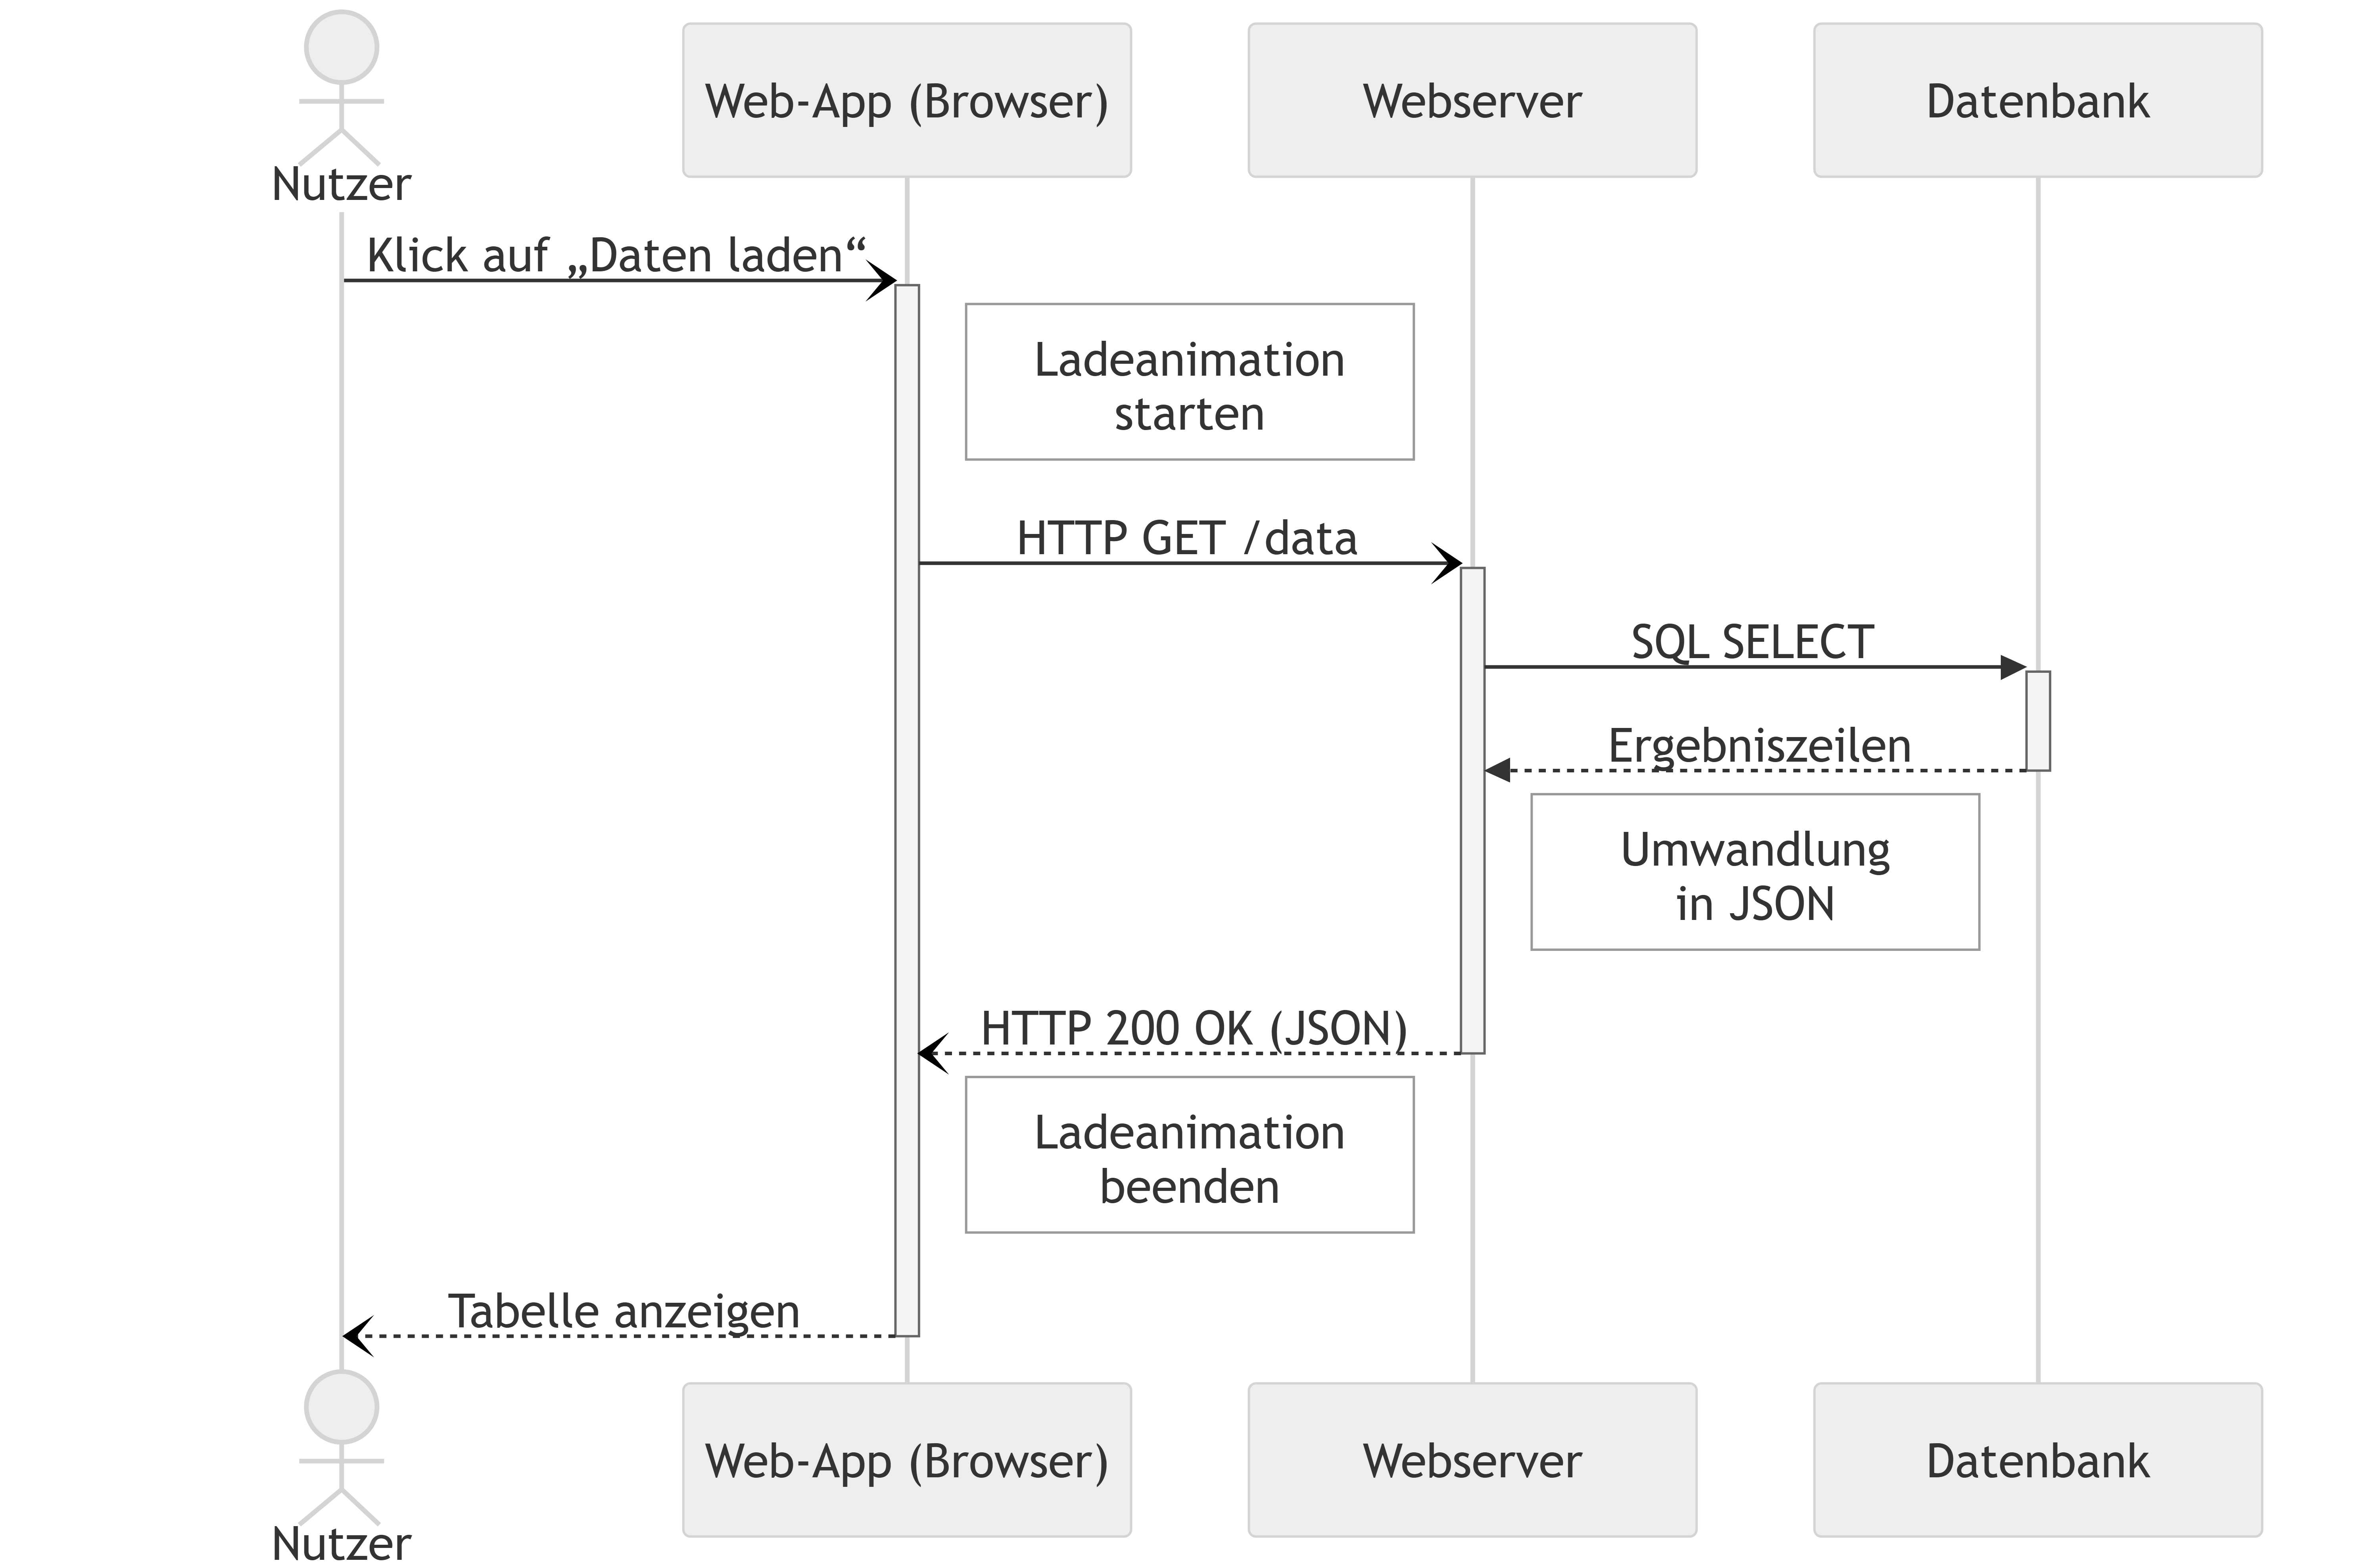
\includegraphics[width=0.9\textwidth]{assets/diagrams/sequenzdiagramm.png}
    \caption{Sequenzdiagramm einer Datenabfrage mit asynchroner HTTP-Anfrage und
        synchronem Datenbankzugriff (Beispiel)}
    \label{fig:sequenz-beispiel}
\end{figure}

% Die beiden folgenden Abschnitte stehen am Ende dieses Kapitels und sind bei
% vielen Prüfern Pflicht.
\section{Verwendete Hard- und Software}
\label{sec:hard-software}
% Komponenten, die im Betrieb der Lösung laufen — mit Versionsangaben
% (Tabelle). Bei Abhängigkeiten mit Versionsbereich die tatsächlich aufgelöste
% Version nennen.

\section{Verwendete Entwicklungs- und Hilfsmittel}
\label{sec:hilfsmittel}
% Entwicklungsumgebung inkl. Erweiterungen, Build- und Diagrammwerkzeuge —
% und SÄMTLICHE KI-Werkzeuge mit Modell und Einsatzzweck. Die Erklärung zur
% Selbständigkeit verweist hierher. Beispieltext unten an die eigene Nutzung
% anpassen; nichts angeben, was nicht tatsächlich genutzt wurde. Die
% Versionen stehen in VS Code unter Erweiterungen bzw. Hilfe > Info.

Als Entwicklungsumgebung diente Visual Studio Code (Version~\dots) mit den
folgenden Erweiterungen:
\begin{itemize}[itemsep=0pt, parsep=0pt, topsep=4pt]
    \item \textit{LaTeX Workshop} (Version~\dots) -- Übersetzung der Ausarbeitung
        mit \texttt{latexmk} und PDF-Vorschau mit SyncTeX,
    \item \textit{Claude Code} (Version~\dots) und das integrierte \textit{GitHub
        Copilot} -- KI-Assistenten im Editor, siehe die Aufstellung der
        KI-Werkzeuge unten,
    \item \textit{Explorer Exclude Manager} (Version~\dots) -- Ausblenden von
        Build- und Hilfsdateien im Dateiexplorer.
\end{itemize}

Als weiteres Hilfsmittel kam \ac{ki} zum Einsatz. Die folgende Aufstellung nennt
die verwendeten Werkzeuge, die dabei genutzten Modelle und den jeweiligen
Einsatzzweck:
\begin{itemize}[itemsep=0pt, parsep=0pt, topsep=4pt]
    \item \textbf{Werkzeug A} (Hersteller, Version) -- Modelle: \dots; Einsatz: \dots
    \item \textbf{Werkzeug B} (Hersteller, Version) -- Modelle: \dots; Einsatz: \dots
\end{itemize}

Sämtliche mit KI-Unterstützung entstandenen Ergebnisse wurden vor der Übernahme
geprüft und überarbeitet; die fachliche Verantwortung für alle Teile der Arbeit
liegt beim Verfasser.

% !TeX root = ../main.tex
\chapter{Implementierung}
\label{cha:implementierung}
% WIE wurde das Konzept umgesetzt? Je Abschnitt benennen, welche
% Anforderungs-IDs er umsetzt.

% !TeX root = ../main.tex
\chapter{Tests und Testergebnisse}
\label{cha:tests}
% Jede Anforderung wird getestet oder ihr Nicht-Test wird begründet. Eine
% Tabelle Anforderungs-ID | Testfall | Ergebnis macht die Durchgängigkeit sichtbar.

% !TeX root = ../main.tex
\chapter{Zusammenfassung und Ausblick}
\label{cha:zusammenfassung}
% Zielerreichung AUSSCHLIESSLICH anhand der dokumentierten Anforderungen
% bewerten. Einschränkungen offen benennen statt kaschieren.


% --- VERZEICHNISSE ---
\clearpage
\chapter{Verzeichnisse}
\label{cha:verzeichnisse}

\printacronyms
% !TeX root = ../main.tex
% Das Quellenverzeichnis ist ein Unterabschnitt des Kapitels "Verzeichnisse".
%
% Die thebibliography-Umgebung von scrreprt setzt ihre Überschrift über
% \chapter*, was einen Seitenumbruch auslöst — die Liste würde von ihrer
% Überschrift getrennt. Innerhalb der Gruppe wird \chapter* daher zum no-op;
% die Überschrift setzt der \section-Befehl, wodurch Nummerierung,
% Inhaltsverzeichnis-Eintrag und PDF-Bookmark regulär entstehen.
\section{Quellenverzeichnis}
\label{sec:quellenverzeichnis}

\begingroup
\makeatletter
\renewcommand{\chapter}{\@ifstar\@gobble\@gobble}
\makeatother
% ieeetr-hm.bst: Ableitung von ieeetr.bst, setzt Titel in Anführungszeichen
% UND kursiv und behält die Groß-/Kleinschreibung aus literatur.bib bei.
% Nummerierung nach Reihenfolge der ersten Nennung im Text.
\bibliographystyle{ieeetr-hm}
\bibliography{literatur}
\endgroup

\listoffigures
\listoftables

\clearpage
% !TeX root = ../main.tex
% Wortlaut der Erklärung mit der Vorlage der eigenen Hochschule abgleichen —
% viele Fakultäten geben ihn verbindlich vor. Der KI-Absatz ist ein Beispiel.
\chapter{Erklärung zur Selbständigkeit}

Ich versichere, dass ich die vorliegende Arbeit selbstständig angefertigt,
keine anderen als die angegebenen Hilfsmittel benutzt, die verwendete Literatur
vollständig aufgeführt sowie Zitate kenntlich gemacht habe. Ich versichere
ferner, dass die Arbeit noch nicht zu anderen Prüfungen vorgelegt wurde.

Der Einsatz von Werkzeugen auf Basis Künstlicher Intelligenz ist als Hilfsmittel
im Sinne dieser Erklärung offengelegt: Die eingesetzten Werkzeuge und ihr
jeweiliger Verwendungszweck sind in \autoref{sec:hilfsmittel} aufgeführt. Die
inhaltliche Verantwortung für alle Teile der Arbeit — einschließlich der von
KI-Werkzeugen unterstützten Passagen — liegt vollständig bei mir; sämtliche
Ergebnisse wurden von mir geprüft, überarbeitet und verantwortet.

\vspace{2cm}

\noindent
\begin{tabular}{@{}p{7cm}p{7cm}@{}}
    \hrulefill & \hrulefill \\
    Ort, Datum & Unterschrift \\
\end{tabular}

% !TeX root = ../main.tex
% Optional. Jeder Anhangsabschnitt braucht mindestens eine Referenz aus dem
% Fließtext (\autoref{sec:anhang-...}), sonst ist er ein Vorgabenverstoß.
\appendix
\chapter{Anhang}
\label{cha:anhang}

\section{Beispiel eines Programmablaufplans}
\label{sec:anhang-pap}

\begin{figure}[H]
    \centering
    % Quelle: assets/diagrams/programmablaufplan.md (Mermaid)
    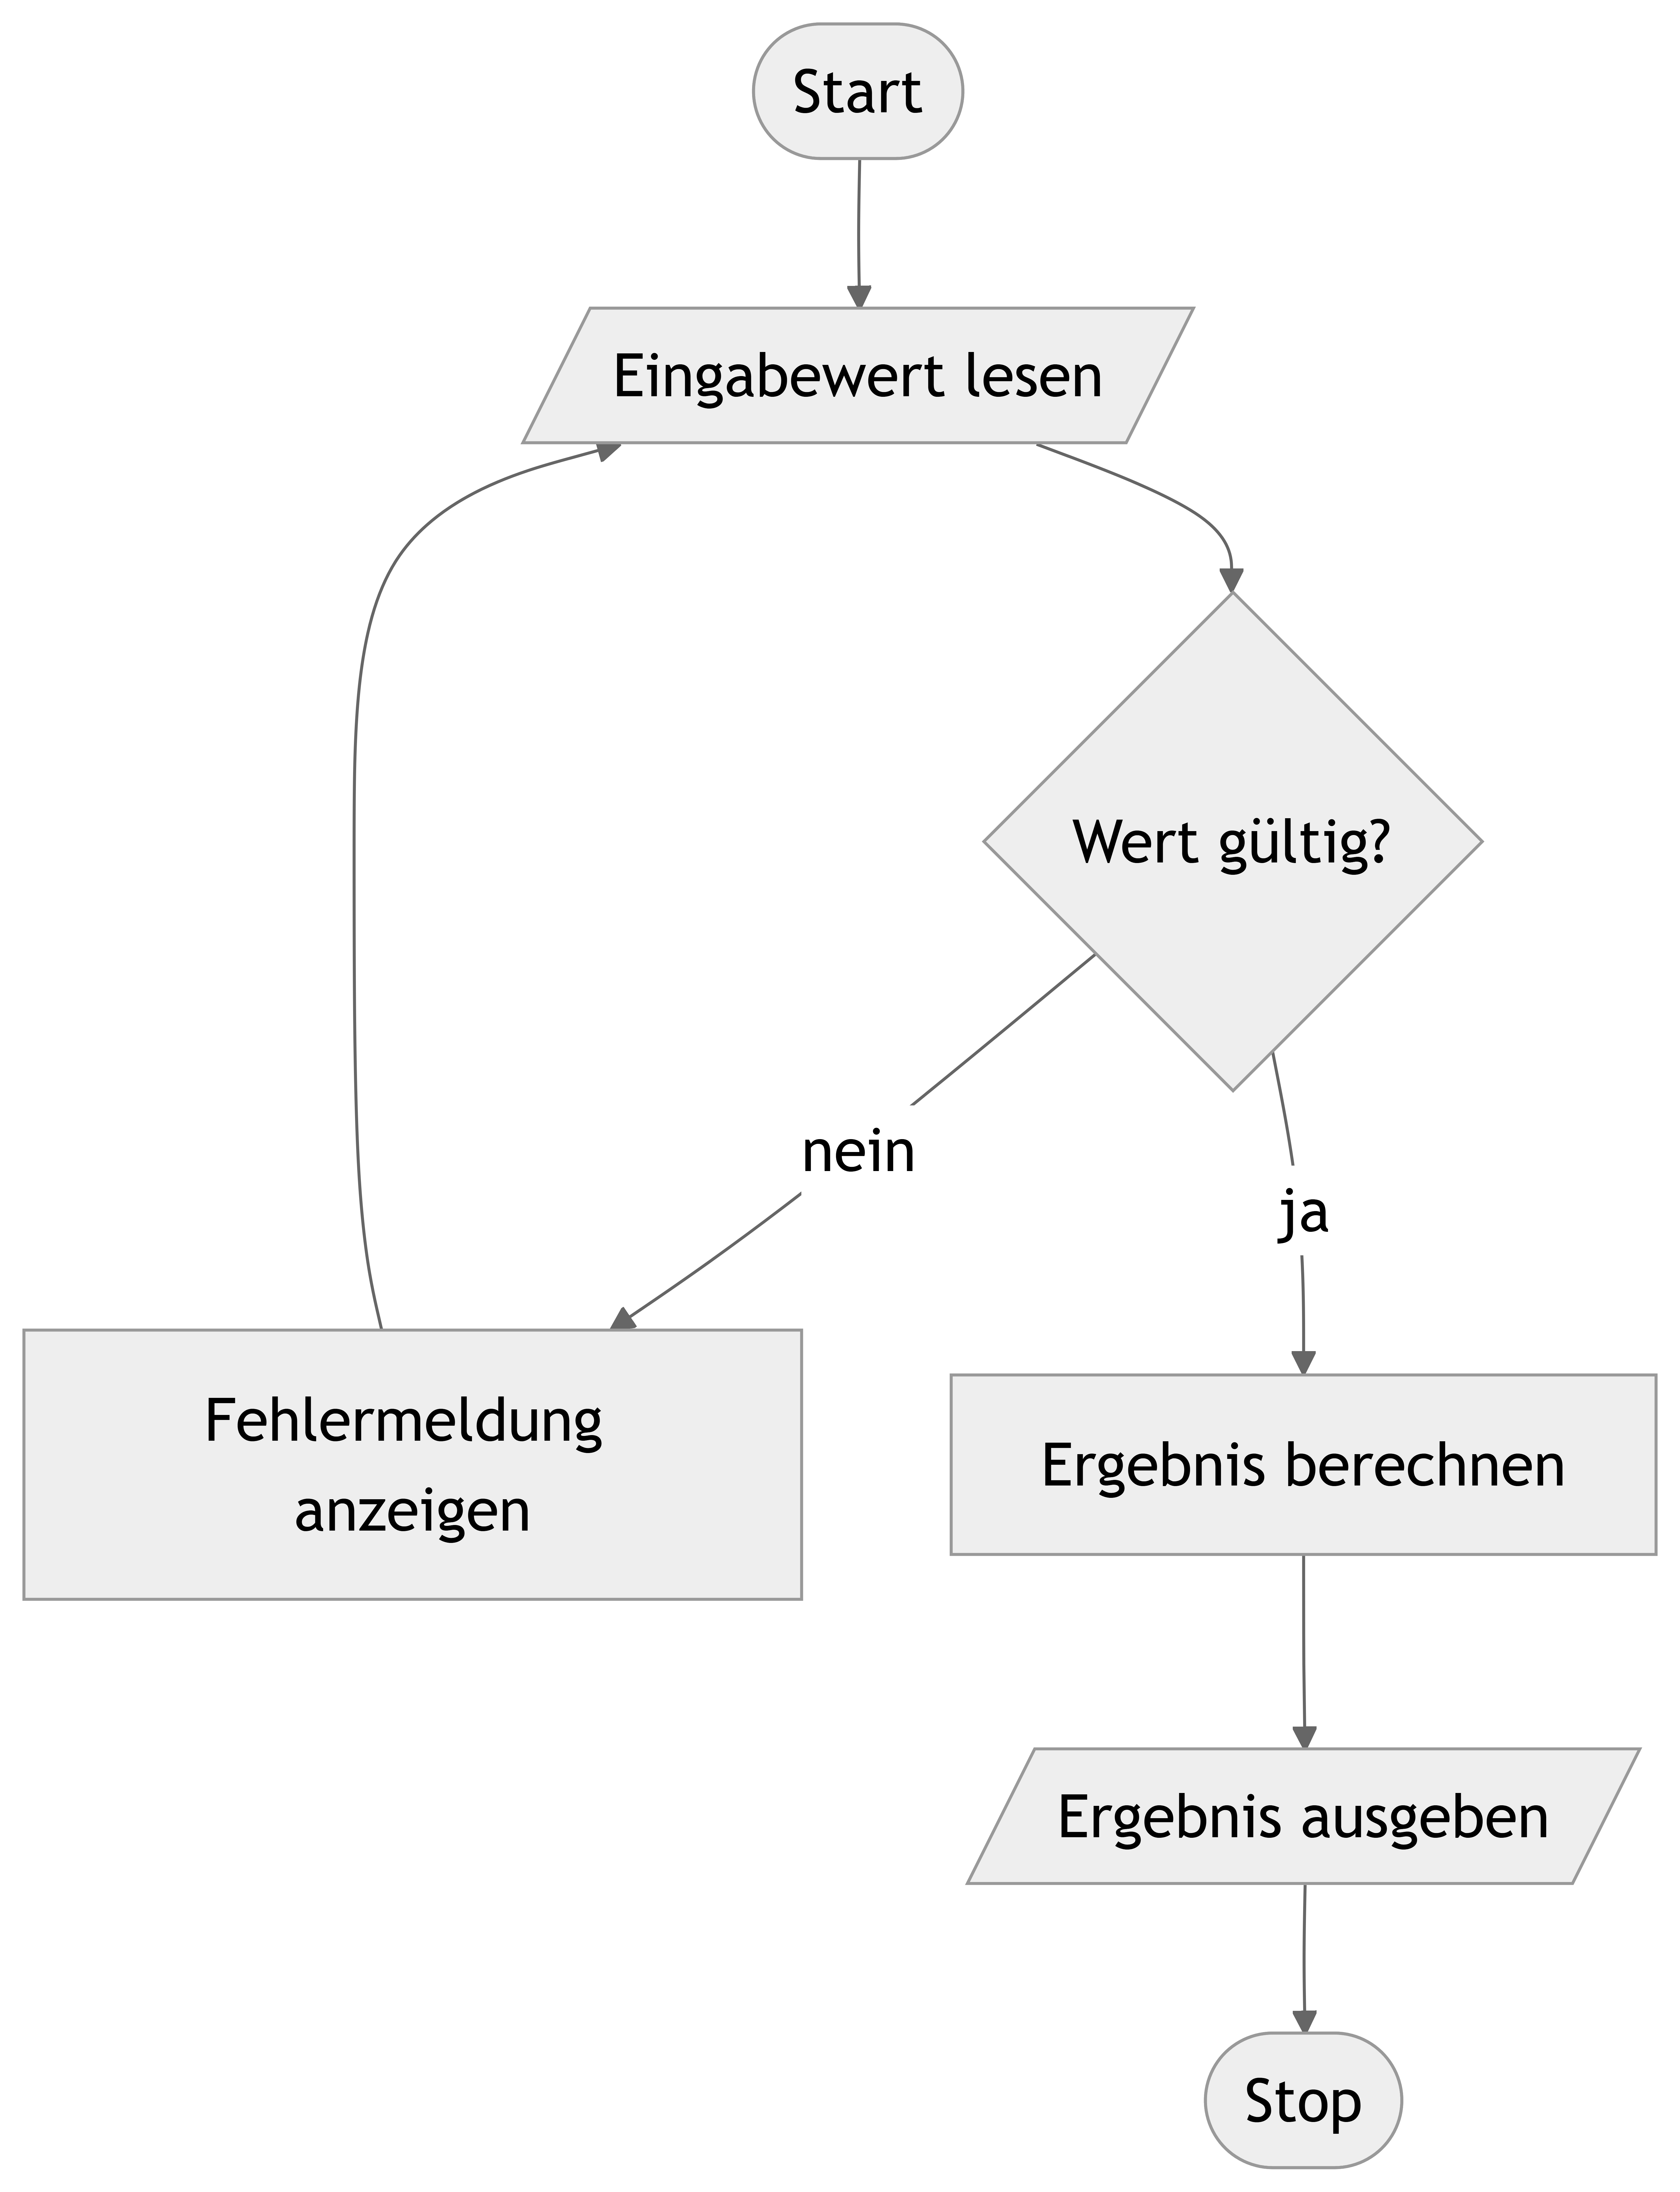
\includegraphics[width=0.6\textwidth]{assets/diagrams/programmablaufplan.png}
    \caption{Programmablaufplan nach DIN~66001 (Beispiel)}
    \label{fig:pap-beispiel}
\end{figure}

\end{document}
